\documentclass[12pt]{report}

%Packages-------------------------------------
\usepackage[svgnames]{xcolor}
\usepackage{amsmath, amsthm, amscd, amsfonts, amssymb}
\usepackage{tikz}
\usepackage{setspace}
\usepackage{wasysym}
\usepackage{framed}
\usepackage{enumitem}
\usepackage{graphics}
\usepackage{graphicx}
\usepackage{cite}
\usepackage[top=25mm, bottom=20mm, left=25mm, right=25mm]{geometry}
%\usepackage[margin=10pt,font=scriprsize,labelfont=bf,labelsep=colon]{caption}
\DeclareGraphicsExtensions{.pdf,.png,.jpg}
%\usepackage{xtocnic}
\usepackage{mathtools}
\usepackage{lipsum}
%\usepackage{perpage}
%‪\usepackage{zref-perpage}



\usepackage{listings}
\lstset{language=R,                                     % set programming language
    basicstyle=\small\ttfamily,                         % basic font style
    stringstyle=\color{DarkGreen},
    otherkeywords={0,1,2,3,4,5,6,7,8,9},
    keywordstyle=\color{Blue},                          % keyword style
    commentstyle=\ttfamily \color{DarkGreen},           % comment style
    backgroundcolor=\color{AliceBlue},                  % background colour
    numbers=left,                                       % display line numbers on the left side
    numberstyle=\ttfamily\color{Gray}\footnotesize,     % line numbers
}

%\usepackage{fontspec}
\tikzstyle{vertex}=[circle, draw, inner sep=0pt, minimum size=6pt]
\newcommand{\vertex}{\node[vertex]}
\usepackage{relsize}
\usepackage[pagebackref=false,colorlinks, linkcolor=blue,citecolor=blue]{hyperref}
\usepackage{xepersian}
\settextfont[Scale=1.3]{XB Zar}
%\MakePerPage[1]{LTRfootnote}
%‪\zmakeperpage{footnote}
\linespread{1.3}
%Layout---------------------------------------
%\DefaultMathsDigits{}


%Commands-------------------------------------
\newcommand\persiangloss[2]{#1\dotfill\lr{#2}\\}


%Theorems-------------------------------------
\newtheorem{thm}{قضیه}[chapter]
\newtheorem{cor}[thm]{نتیجه}
\newtheorem{defn}[thm]{تعریف}
\newtheorem{prop}[thm]{گزاره}
\newtheorem{lmm}[thm]{لم}
\newtheorem{conj}[thm]{حدس}
\newtheorem{exm}[thm]{مثال}
\newtheorem{rem}[thm]{تذکر}
\newtheorem{note}[thm]{یادداشت}
\newtheorem{alg}[thm]{الگوریتم}

%\settextfont[Scale=1.2]{XB Niloofar}
%\setlatintextfont[Scale=2]{Linux Libertine}
%\setlatintextfont[Scale=1]{Times New Roman}
% از revision 118 زی‌پرشین به بعد، وارد کردن دستور زیر لازم نیست. توجه داشته باشید که در صورت  غیرفعال کردن این دستور،
% از فونت پیش‌فرض لاتک برای کلمات انگلیسی استفاده خواهد شد.
%\setlatintextfont[ExternalLocation,BoldFont={lmroman10-bold},BoldItalicFont={lmroman10-bolditalic},ItalicFont={lmroman10-italic}]{lmroman10-regular}
% چنانچه می‌خواهید اعداد در فرمول‌ها، فارسی باشد، خط زیر را نیز فعال کنید
%\setdigitfont[Scale=1.2]{XB Zar}
%%%%%%%%%%%%%%%%%%%%%%%%%%
% تعریف قلم‌های فارسی و انگلیسی برای استفاده در بعضی از قسمت‌های متن
%\defpersianfont\titr[Scale=1.2]{XB Titre}
\defpersianfont\nastaliq[Scale=2]{IranNastaliq}
%\defpersianfont\traffic[Scale=1]{B Traffic}
% چنانچه فونت B Traffic را ندارید، دستور بالا را غیرفعال کرده و دستور زیر را فعال کنید
%\defpersianfont\traffic[Scale=1.3]{B Yas}
%%%%%%%%%%%%%%%%%%%%%%%%%%
%تعریف و نحوه ظاهر شدن عنوان قضیه‌ها، تعریف‌ها، مثال‌ها و ...
\renewcommand{\listfigurename}{فهرست شکل‌ها}
%\includegraphics[scale=1]{fig_name}
%\newcommand{\bR}{\mathbb{R}}
%\newcommand{\bF}{\mathcal{F}}
%\theoremstyle{definition}
%\newtheorem{definition}{تعریف}[chapter]
%\newtheorem{theorem}{قضیه}[chapter]
%\newtheorem{lemma}{لم}[chapter]
%\newtheorem{lemma}[definition]{لم}
%\newtheorem{proposition}{گزاره}
%\newtheorem{corollary}{نتیجه}[chapter]
%\newtheorem{remark}{ملاحظه}
%\newtheorem{Point}{نکته}
%\newtheorem{example}{مثال}[chapter]
%\newcommand{\bl}{\begin{lemma}}
%\newcommand{\el}{\end{lemma}}
%\newcommand{\iid}{\mbox{$\displaystyle \begin{array}{c}\mbox{\tiny\bf $i.i.d.$}\\ \mbox{\huge $\sim$}\vspace{0.3cm}\end{array}$}}
%\newcommand{\p}{\mbox{$\displaystyle \begin{array}{c}\mbox{\tiny\bf $P$}\\ \mbox{\huge $\longrightarrow$}\vspace{0.3cm}\end{array}$}}
%\newcommand{\dd}{\mbox{$\displaystyle \begin{array}{c}\mbox{\tiny\bf $d$}\\ \mbox{\huge $\longrightarrow$}\vspace{0.3cm}\end{array}$}}
%\newcommand{\bp}{\begin{proof}}
%\newcommand{\ep}{\end{proof}}
%\newcommand{\Z}{\mathbb{Z}}
%\newcommand{\R}{\mathbb{R}}
%\newcommand{\integ}{\int_{-\infty}^{+\infty}}
%\settextfont[Scale=1.14]{B Zar}
%\setdigitfont[Scale=1.14]{B Zar}
%دستوری برای تعریف واژه‌نامه
\newcommand\gloss[2]{#2\dotfill\lr{#1}\\}
% تغییر نام کلمه «اثبات» به «برهان»
%\renewcommand\proofname{\textbf{برهان}}
% دستوری برای تغییر نام کلمه «کتاب‌نامه» به «مراجع»
%\renewcommand{\bibname}{مراجع}
% دستوری برای تعریف واژه‌نامه انگلیسی به فارسی
%\newcommand\persiangloss[2]{#2\dotfill\lr{#1}\\}
% دستوری برای تعریف واژه‌نامه فارسی به انگلیسی
%\newcommand\englishgloss[2]{#2\dotfill\lr{#1}\\}


% دستورهایی برای ایجاد کادر (جعبه)
%\newenvironment{fminipage}
%{\begin{Sbox}\begin{minipage}}
%{\end{minipage}\end{Sbox}\fbox{\TheSbox}}
%\setlength\belowcaptionskip{0pt}
%\setlength\abovecaptionskip{0pt}


\begin{document}
\thispagestyle{empty}
\pagenumbering{adadi}
\begin{figure}
\centering

\includegraphics[scale=1.2]{bh}
\end{figure}

%Title page ---------------------------------------------
\thispagestyle{empty}
\begin{figure}
\centering
\includegraphics[scale=0.1]{UT-Logo.png}
\end{figure}

\begin{center}
{\small دانشگاه تهران
\\
مرکز تحقیقات بیوشیمی-بیوفیزیک}
\end{center}

\vfill

\begin{center}

\LARGE{\textbf{عنوان پایان‌نامه }}
\end{center}
\vfill
\begin{center}
نگارش\\
{\large
\textbf{نام و نام خانوادگی دانشجو}}
\end{center}
\begin{center}
استاد(های) راهنما \\

{\large \textbf{نام و نام خانوادگی استاد(های) راهنما}}
\end{center}
\begin{center}
استاد مشاور \\

{\large \textbf{در صورت وجود}}
\end{center}



\vfill
{\small
\begin{center}
 پایان‌نامه برای دریافت درجه دکترا
\\
در رشته بیوانفورماتیک
\end{center}

\begin{center}
تاریخ 
\end{center}
}
\pagestyle{empty}
\pagenumbering{}


%\pagestyle{headings}\input{taqdim_nameh}
%\setcounter{page}{1}
%\pagenumbering{roman}
\pagestyle{plain}
\setcounter{page}{1}
\pagenumbering{adadi}
%Abstract page-------------------------------

%Dedication page-----------------------------

\clearpage
\thispagestyle{empty}
\begin{flushright}
\begin{nastaliq}
\begin{Huge}
تقديم به
\end{Huge}
\end{nastaliq}
\end{flushright}
\vskip 1cm
\qquad 
\begin{nastaliq}
\begin{huge}
\quad 
\begin{flushright}
\quad  ....\\
\vskip 1cm
\quad \\
\vskip 1cm
 \quad  \\
\end{flushright}

\end{huge}
\end{nastaliq}

%Acknowledgement page------------------------
\clearpage
\thispagestyle{empty}
\begin{flushright}
\begin{nastaliq}
\begin{Huge}
سپاسگزاری...
\end{Huge}
\end{nastaliq}
\end{flushright}
\vskip 1cm
\qquad 
\begin{nastaliq}
\begin{large}
\quad 
\begin{flushright}
سپاس از ...\\[0.5cm]
\quad 
و همچنين سپاس از ا....\\
\vskip 1cm
\quad \\
\vskip 1cm
 \quad  \\

\end{flushright}
\begin{flushleft}
نام و نام خانوادگی\\
فصل سال
\end{flushleft}
\end{large}
\end{nastaliq}

%copyright + declaration page
\chapter*{تعهدنامه اصالت اثر}
%\section*{اصالت اثر}
اينجانب  ..........................متعهد مي شوم كه مطالب مندرج در اين پايان نامه/رساله حاصل كار پژوهشي اينجانب است و به دستاوردهاي پژوهشي ديگران كه در اين پژوهش از آنها استفاده شده است، مطابق مقررات ارجاع و در فهرست منابع و مآخذ ذكر گرديده است. اين پايان نامه/رساله قبلاً براي احراز هيچ مدرك هم سطح يا بالاتر ارائه نشده است. در صورت اثبات تخلف (در هر زمان) مدرك تحصيلي صادر شده توسط دانشگاه از اعتبار ساقط خواهد شد. 
كليه حقوق مادي و معنوي اين اثر متعلق به دانشكده ریاضی، آمار و علوم کامپیوتر دانشکدگان علوم دانشگاه تهران مي باشد. 
\begin{flushleft}
نام و نام خانوادگی
امضا 
\end{flushleft}

\chapter*{حق مالکیت معنوی}
%\section*{حق مالکیت معنوی}
حق مالکیت معنوی این اثر متعلق به دانشگاه تهران می‌باشد. استفاده از مطالب این پایان‌نامه در فعالیت‌های تحقیقاتی با ذکر منبع بلامانع می‌باشد. در صورت استفاده تجاری، مانند چاپ این پایان‌نامه، هماهنگی لازم و اجازه کتبی از دانشگاه و نگارنده پایان‌نامه الزامی می‌باشد.
%\listoffigures
\chapter*{خروجی‌های پايان‌نامه}
\begin{latin}
\begin{enumerate}
\item 
paper1
\item 
paper2
\end{enumerate}
\end{latin}
%-------------------------
%\pagestyle{plain}
%\setcounter{page}{1}
%\pagenumbering{harfi}
%-------------------------

%\listoftables

\begin{abstract}
چکیده پایان‌نامه باید شامل نتایج اصلی مورد مطالعه باشد. توجه نمایید که چکیده با پیشگفتار تفاوت دارد و محلی برای طرح مبانی یا مفاهیم مقدماتی نیست. چکیده تنها باید شامل نتایج و کار اصلی انجام شده در پایان‌نامه باشد. طول چکیده معمولاً بیشتر از یک یا دو پاراگراف نیست.
\\

\textbf{کلمات کلیدی: }کلمات اصلی که در موضوع و متن پایان نامه استفاده شده‌اند و ترجیحاً در چکیده و عنوان نیستند که با کاما از هم جدا شده باشند

\end{abstract}\addcontentsline{toc}{chapter}{چكيده}

\chapter*{پیشگفتار }

پیش‌گفتار، فصلی از پایان‌نامه است که معمولاً شامل بخش یا زیربخش نیست و حدود یک یا دو صفحه است. در آن، مقدمه‌ای به زبان ساده و عاری از فرمول‌بندی ریاضی، از مساله مورد مطالعه در پایان‌نامه ارائه می‌شود. همچنین در پیش‌گفتار است که می‌توان خواننده را با تاریخچه‌ای مختصر از تلاش‌هایی که برای حل مساله مورد مطالعه در پایان‌نامه شده است آشنا نمود و نیز تلاش نمود تا خواننده اهمیت کار انجام شده در پایان‌نامه را دریابد. این قسمت، گرچه در نگاه نخست به ظاهر بسیار ساده می‌نماید، اما در حقیقت یکی از  مهمترین قسمت‌های پایان‌نامه است، زیرا بازتاب دهنده دانسته‌ها و فهم دانشجو از کلیت مساله است. توصیه می‌کنیم که نوشتن این قسمت را به آخر موکول نمایید!
\\
یک نکته مهم: اگر پایان‌نامه بر اساس یک یا چند مقاله نوشته شده است، آنگاه از دانشجو انتظار می‌رود که مراجع اصلی خود را در پیش‌گفتار معرفی نماید.
\\
معمولاً بخش آخر پیش‌گفتار به ارائه یک نمایه کلی از پایان‌نامه اختصاص می‌یابد و نگارنده در پاراگراف‌های مجزا، به معرفی کوتاهی از فصل‌بندی و کار انجام شده در هر فصل پایان‌نامه می‌پردازد.

 

\addcontentsline{toc}{chapter}{پيشگفتار}

\tableofcontents\addcontentsline{toc}{chapter}{فهرست مطالب}

\listoffigures\addcontentsline{toc}{chapter}{فهرست شكل‌ها}

\listoftables\addcontentsline{toc}{chapter}{فهرست جداول}
%---------------------

%---------------------

%\part{مفاهيم و تعاريف مقدماتي}
\chapter{
مفاهیم مقدماتی
}\label{S1}
\setcounter{page}{1}
\pagenumbering{arabic}

فصل اول پایان‌نامه به بیان تعاریف و مفاهیم اولیه اختصاص دارد.  معمولاً نمادگذاری و معرفی کلیدواژه‌های به کار رفته در پایان‌نامه در این فصل انجام می‌پذیرد و خواننده در صورت عدم آشنایی با مفهومی، می‌تواند به این فصل مراجعه نماید.

 توجه کنید که لزومی به اثبات همه مطالب و قضیه‌های مقدماتی، در این فصل، نیست و اصولاً چنین کاری شیوه مرسوم نیست. معمولاً انتخاب و ارجاع خواننده به یک کتاب معتبر یا هر مرجع معتبر دیگری بسیار مناسب‌تر است. چنین فصلی، جایی مناسب برای قضیه‌های «کلاسیک» درباره مساله مورد مطالعه است. توجه کنید که یک قضیه می‌تواند صورت‌های مختلفی داشته باشد و بهتر است از آن صورت مورد استفاده خود در این قسمت استفاده نمایید!

تعداد صفحات متوسط برای هر فصل بین 15 تا 25 صفحه و تعداد صفحات معمول برای پایان‌نامه بین 70 تا 100 صفحه است. 
به طور معمول پایان‌نامه‌های استاندارد دارای 4 یا 5 فصل هستند که در فصل اول مقدمات، در فصل‌های دوم و سوم مطالب نظری اصلی و در فصل چهارم برای رشته هایی نظیر آمار، آزمایش‌های عددی و تحلیل داده‌ها آورده می‌شود. فصل پنجم می‌تواند یک فصل کوتاه دو یا سه صفحه‌ای شامل جمع‌بندی، نتیجه‌گیری و پیشنهادات آینده باشد. 

برای زیرنویس معمولا از دستوری به این صورت\LTRfootnote{\lr{A footnote}} استفاده می‌شود. تعداد زیرنویس‌ها نبایستی خیلی زیاد باشد و بهتر است تنها به عنوان‌های تخصصی زیرنویس داد و مابقی واژگان را در بخش واژه‌نامه فارسی به انگلیسی  در انتهای پایان‌نامه آورد. فرمول‌های داخل متن به عنوان نمونه به صورت 
 $\{{Y_t}\}_{t=1}^T$
و فرمول‌های بین خط‌ها به عنوان نمونه به صورت زیر می‌آیند
\begin{equation}\label{graph_model}
\Pr(\mathbf{s},\mathbf{y})=\Pr(s_1)\Pr(y_1|s_1)\prod_{t=2}^{T}\Pr(s_t|s_1,\dots,s_{t-1})\Pr(y_t|y_1,\dots,y_{t-1},s_1,\dots,s_{t})
\end{equation}
و برای ارجاع دادن به این فرمول‌ از 
\eqref{graph_model} استفاده می‌شود. رعایت نیم‌فاصله‌ها در تمامی متن توصیه می‌شود. 
همچنین نقطه و کاما بایستی چسبیده به انتهای کلمه ماقبل و با فاصله از ابتدای کلمه بعد باشند. 

برای شروع یک پاراگراف جدید حتما بایستی یک خط فاصله خالی بین پاراگراف قبلی و بعدی بگذارید. برای آوردن شکل به صورت شکل 
\ref{fig.hmm}
عمل می‌کنیم. 
\begin{figure}[h!]
\centering
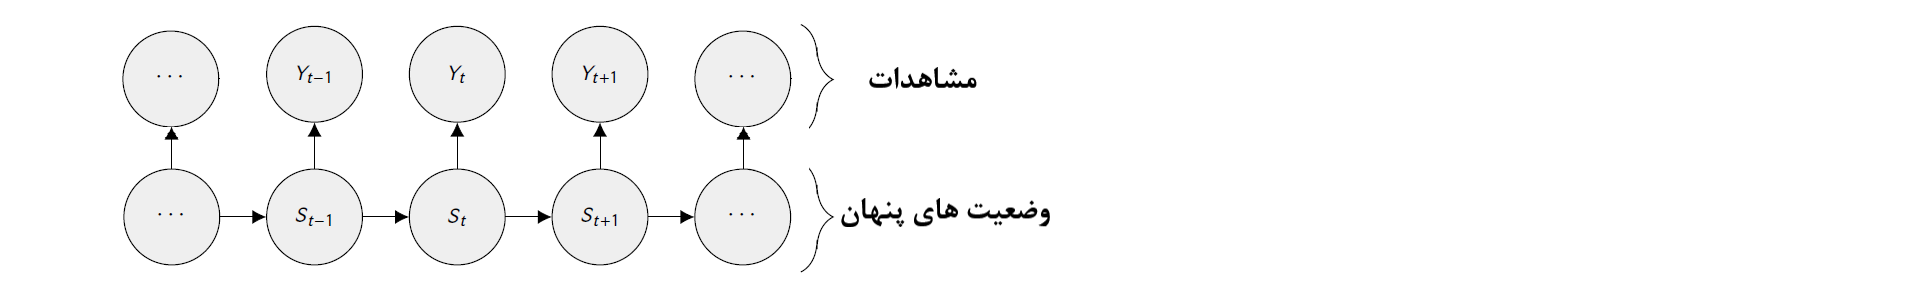
\includegraphics[scale=0.7]{HMM}
\caption{مصورسازی گرافی یک مدل مارکوف پنهان}
\label{fig.hmm}
\end{figure}

توجه کنید که اگر شکل را از منبعی به امانت گرفته‌اید بایستی حتما در زیرنویس شکل به آن منبع ارجاع دهید. 

برای ایجاد یک بخش جدید به صورت زیر عمل می‌کنیم. 

\section{بخش}

همینطور از نماد دو نقطه در فارسی تنها برای لیستی به صورت زیر استفاده می‌شود و قبل از فرمول‌ها استفاده از دونقطه توصیه نمی‌شود:
\begin{enumerate}
\item مورد اول
\item    مورد دوم ...
\end{enumerate}

برای ایجاد یک فرمول چند خطی می‌توانید به صورت زیر عمل کنید

\begin{align}
A &= B \nonumber \\ 
   & = C \label{alignformula}
\end{align}

برای ارجاع دادن به یک مرجع در متن به عنوان نمونه می‌توان به صورت 
 \cite{langrock2015b,pohle2017} عمل کرد.


\begin{defn}
عدد طبیعی 
$p$، 
$p\neq 1$، 
را اول گوییم، هرگاه به غیر از خودش و یک مقسوم علیه دیگری نداشته باشد.
\end{defn}


در این بخش یک شکل دیگر نیز برای نمونه می‌آوریم تا فهرست شکل‌ها کمی پربارتر باشد. 
\begin{figure}
\centering
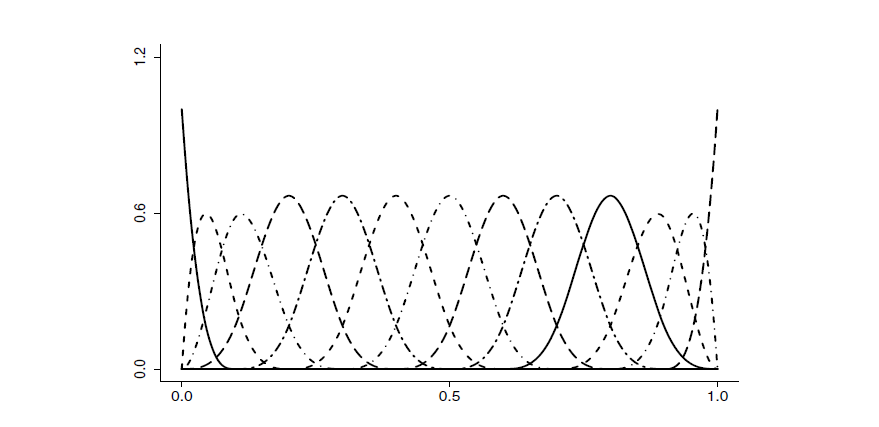
\includegraphics[scale=0.8]{spline}
\caption{پايه \lr{B}-اسپلاين درجه سه با استفاده از نه گره با فاصله‌هاي برابر در بازه $ (0,1) $}
\end{figure}

گاهی نیاز دارید تا یک شکل باکیفیت را در خود لاتک ایجاد کنید. نمونه‌ای از این کار در شکل 
\ref{spline-graph}
آورده شده است. توجه کنید که ارجاع به فرمول‌ها با پرانتز و ارجاع به شکل‌ها و جدول‌ها بدون پرانتز است. 

\begin{figure}
\centering
\begin{tikzpicture} [scale=2, thick]

\vertex[fill, scale = 2] (B11) at (2,2) [label=above:$B_{1,1}$] {};
\vertex[fill, scale = 2] (B21) at (2,1) [label=above:$B_{2,1}$] {};
\vertex[fill, scale = 2] (B31) at (2,0) [label=above:$B_{3,1}$] {};
\vertex[fill, scale = 2] (B41) at (2,-1) [label=above:$B_{4,1}$] {};
\vertex[fill, scale = 2] (B51) at (2,-2) [label=above:$B_{5,1}$] {};

\vertex[fill, scale = 2] (B12) at (3,1.5) [label=above:$B_{1,2}$] {};
\vertex[fill, scale = 2] (B22) at (3,0.5) [label=above:$B_{2,2}$] {};
\vertex[fill, scale = 2] (B32) at (3,-0.5) [label=above:$B_{3,2}$] {};
\vertex[fill, scale = 2] (B42) at (3,-1.5) [label=above:$B_{4,2}$] {};

\vertex[fill, scale = 2] (B13) at (4,1) [label=above:$B_{1,3}$] {};
\vertex[fill, scale = 2] (B23) at (4,0) [label=above:$B_{2,3}$] {};
\vertex[fill, scale = 2] (B33) at (4,-1) [label=above:$B_{3,3}$] {};

\vertex[fill, scale = 2] (B14) at (5,0.5) [label=above:$B_{1,4}$] {};
\vertex[fill, scale = 2] (B24) at (5,-0.5) [label=above:$B_{2,4}$] {};

\path
(B11) edge[-to] (B12)
(B21) edge[-to] (B12)
(B21) edge[-to] (B22)
(B31) edge[-to] (B22)
(B31) edge[-to] (B32)
(B41) edge[-to] (B32)
(B41) edge[-to] (B42)
(B51) edge[-to] (B42)
(B12) edge[-to] (B13)
(B22) edge[-to] (B13)
(B22) edge[-to] (B23)
(B32) edge[-to] (B23)
(B32) edge[-to] (B33)
(B42) edge[-to] (B33)
(B13) edge[-to] (B14)
(B23) edge[-to] (B14)
(B23) edge[-to] (B24)
(B33) edge[-to] (B24);
\end{tikzpicture}
\caption{نمايي از معادله بازگشتي تابع پايه \lr{B}-اسپلاين درجه 4}
\label{spline-graph}
\end{figure}



%\part{مدل‌هاي تبديل ماركوفي ناپارامتري}
\chapter{عنوان فصل}\label{S2}
\pagestyle{plain}

در این فصل به مطالب اصلی نظری پایان‌نامه پرداخته می‌شود. ممکن است در این فصل هنوز به مدل‌های اصلی و ایده‌های اصلی مقاله اصلی پایان‌نامه اشاره نشود، ولی دیگر مفاهیم و تعاریف اولیه در این فصل گفته نمی‌شوند و بیش‌تر این فصل می‌تواند در برگیرنده قضایا و مطالب پژوهشی و یا شرح مدل‌های قبلی و روش‌های پیشین باشند که قرار است با روش نظری مقاله اصلی مقایسه شوند. البته این مساله در رشته‌های گوناگون می‌تواند متفاوت باشد ولی در کل شباهت‌هایی بین ساختارهای گوناگون در رشته‌های گوناگون از این منظر وجود دارد. 

























\chapter{عنوان فصل}\label{S3}
\pagestyle{plain}


فصل سوم معمولا اوج پایان‌نامه و پرداختن به مطالب اصلی مقاله اصلی پایان‌نامه است. 


%\part{نتايج و پيشنهادات آينده}
\chapter{عنوان فصل}\label{S4}
\pagestyle{plain}


 در این فصل به مطالب تکمیلی و اثبات‌های قضایای اصلی و یا کاربردها پرداخته می‌شود. 
 
 در رشته هایی نظیر آمار، این فصل بیش‌تر به تحلیل داده‌ها، شبیه‌سازی و یا مثال‌های عددی می‌پردازد و می‌تواند عنوانی مانند "آزمایش‌های عددی و تحلیل داده‌ها" داشته باشد. در این فصل معمولا جدول‌هایی نیز آورده می‌شود که نمونه‌ای از آن در جدول 
\ref{res1}
آورده شده است. این جدول‌ها در فهرست جدول‌ها آورده می‌شوند. 

\begin{table}[h!]
\centering
\begin{tabular}{c|c|c|c}
%\hline
توزیع گسیل&همگنی (\%)&\lr{AIC}&\lr{BIC}\\[0.1cm]
\hline\hline
ناپارامتري&86/2, 88/9, 80&6419/063&6805/525\\[0.3cm]
%\hline
نرمال&58/3,99/1,81/1&7560/346&7661/162\\[0.3cm]
%\hline
نرمال آميخته&58/3,99/1,81/1&7593/376&7795/008\\
\end{tabular}
\caption{جدول مقايسه توزيع گسيل ناپارامتري و نرمال و نرمال آميخته در مدل ماركوف پنهان}
\label{res1}
\end{table}


انتظار می‌رود در این فصل تمامی جنبه‌های عددی روش‌های ارائه شده بررسی شده و این روش‌ها با روش‌های دیگر بر اساس ملاک‌های گوناگون مقایسه شوند. 



\chapter{نتیجه‌گیری و جمع‌بندی}\label{S5}
\pagestyle{plain}


در اين فصل، ابتدا به جمع‌بندي مباحث مطرح‌ شده در مورد روش‌های مورد مطالعه می‌پردازيم. سپس براي پژوهش‌های آينده پيشنهادهايی را مطرح خواهيم كرد كه می‌تواند براي پژوهش‌گران علاقه‌مند به اين حوزه براي توسعه روش‌های جديدتر يا استفاده از روش‌های موجود در چالش‌هاي كاربردی ديگر ارائه دهد.
\section{جمع‌بندی}

در این بخش یک جمع‌بندی از مطالب پایان‌نامه و نتایج ارائه می‌شود. 

\section{پيشنهادات}
در ادامه برخی پيشنهادات براي مطالعات آينده ارائه می‌شود.


























\linespread{2}
\bibliographystyle{abbrv}
\renewcommand{\bibname}{\rl{{مراجع}\hfill}}
\lr{\bibliography{references}}
\addcontentsline{toc}{chapter}{مراجع}

\linespread{1}
\chapter*{پيوست: كدهاي \texttt{R}}
\addcontentsline{toc}{chapter}{پيوست: كدهاي \texttt{R}}
\begin{latin}
\begin{lstlisting}[title={\large Nonparametric M-step}] 
rm(list = ls())
library(psych)
library(cpr)
library(MASS)
nonpar_mstep = function (x, wt,
 control = list(K = 5, lambda0 = 0.5)) 
{
  defcon <- list(K = 5, lambda0 = 0.5)
  control <- modifyList(defcon, control)
  K <- control$K
  lambda0 <- control$lambda0
  nstate <- ncol(wt)
  emission <- list(coef = list())
  lambda <- numeric(nstate)
  d <- ncol(x)
  n <- nrow(x)
  tryCatch({
    a <- matrix(0, nrow = n, ncol = K^d)
    if (object.size(a) > 1.8e+09) 
      warning("The dimension of the data or 
              the degree of the spline is large!
              \n\t\tThis will result in a very slow progress!")
    rm(a)
  }, error = function(cond) {
    stop("The dimension of the data or
         the degree of the spline is too large!
         \n\t\tThere is no enough memory for fitting!
         Try another emission distribution.")
  })
  basis = btensor(lapply(1:d, function(i) x[, i]), df = K, 
                  bknots = lapply(1:d, function(i)
                    c(min(x[, i]) - 0.01,
                      max(x[, i]) + 0.01)))
  for (j in 1:nstate) {
    lambda[j] <- lambda0
    mloglike_lambda0 <- function(beta) {
      dbeta <- diff(beta, differences = 2)
      omega <- exp(beta)/sum(exp(beta))
      loglike <- t(wt[, j]) %*% log(basis %*% omega) - 
        lambda0/2 * sum(dbeta^2)
      return(-loglike)
    }
    start <- runif(K^d)
    suppressWarnings(fit <- nlm(mloglike_lambda0, start, 
                                hessian = T))
    H_lambda0 <- -fit$hessian
    difference <- 1
    eps <- 1e-06
    cntr <- 1
    beta_hat <- list(rep(1, K))
    while (difference > eps) {
      mloglike <- function(beta) {
        dbeta <- diff(beta, differences = 2)
        omega <- exp(beta)/sum(exp(beta))
        inf_index <- which(is.infinite(log(basis %*% 
                                             omega)))
        loglike <- t(wt[, j]) %*% log(basis %*% omega) - 
          lambda[j]/2 * sum(dbeta^2)
        return(-loglike)
      }
      start <- runif(K^d)
      suppressWarnings(fit <- nlm(mloglike, start, hessian = T))
      H <- -fit$hessian
      beta_hat[[cntr + 1]] <- fit$estimate
      df_lambda <- tr(ginv(H) %*% H_lambda0)
      dbeta <- diff(beta_hat[[cntr + 1]], differences = 2)
      lambda[j] <- (df_lambda - d)/(sum(dbeta^2))
      difference <- sum(beta_hat[[cntr + 1]] - beta_hat[[cntr]])
      cntr <- cntr + 1
    }
    emission$coef[[j]] <- exp(beta_hat[[cntr]])/
      sum(exp(beta_hat[[cntr]]))
  }
  emission
}
\end{lstlisting}
\end{latin}


\chapter*{واژه‌نامه فارسی - انگلیسی }
\addcontentsline{toc}{chapter}{واژه‌نامه فارسی - انگلیسی}
\persiangloss{الگوريتم پسرو}{Backward Algorithm}
\persiangloss{تابع پله‌اي}{Step Function}
\persiangloss{ماتريس احتمال انتقال}{Transition Probability Matrix}



\begin{latin}
\begin{abstract}
The English abstract should match the persion one once traslated.\\[0.5cm]
\textbf{Keywords: } The english keywords should match the persian ones once translated. 
\end{abstract}
\newpage

%Title page ---------------------------------------------
\pagenumbering{gobble}
\begin{figure}
\centering
\includegraphics[scale=0.1]{UT-Logo.png}
\end{figure}
\begin{center}
University of Tehran\\
Institute of Biochemestry and Biophysics
\end{center}

\vfill

\begin{center}
\LARGE{Insert the english title of the dissertation}
\end{center}

\vfill

{\large \begin{center}
\textbf{
By\\
} Insert your name and surname here 
\end{center}

\begin{center}
\textbf{Supervisor(s)\\} Insert the name(s) of supervisor(s) here
\end{center}

\begin{center}
\textbf{Advisor\\} Insert the name(s) of Advisor here
\end{center}

}
\vfill
\begin{center}
{\small A thesis submitted to graduate studies office
in partial fulfillment of the requirements for the degree of master of science in Mathematics and Applications / Applied Mathematics /
Statistics / Computer Science}
\end{center}

\begin{center}
Date
\end{center}

%\pagestyle{empty}
%\pagenumbering{}

\end{latin}
\end{document}
